\documentclass{beamer}

\usepackage[utf8]{inputenc}
\usepackage[T1]{fontenc}
\usepackage[french]{babel}
\usepackage[babel=true]{csquotes} % guillements français
\usepackage{graphicx}
\graphicspath{{Images/}}
\usepackage{color}
\usepackage{hyperref}
\hypersetup{colorlinks,linkcolor=,urlcolor=blue}
\usepackage{listings}


\mode<presentation>
{
  %% PLUSIEURS THEMES EXISTENT : VOIR DOCUMENTATION
  % \usetheme{Warsaw}
  % \usetheme{Frankfurt}
  \usetheme{Madrid}
  % or ...

  \setbeamercovered{transparent}
  % or whatever (possibly just delete it)
}


\title[Dev. Mobiles -- L3 info]{UnivMap\\L3 informatique}
\author{Damien Laoussing Dylan Cherrier}
\institute[DI]{Département d'informatique}
\date{\today}


\subject{Talks}
% This is only inserted into the PDF information catalog. Can be left
% out.



% If you have a file called "university-logo-filename.xxx", where xxx
% is a graphic format that can be processed by latex or pdflatex,
% resp., then you can add a logo as follows:

% \pgfdeclareimage[height=0.5cm]{university-logo}{university-logo-filename}
% \logo{\pgfuseimage{university-logo}}



% Delete this, if you do not want the table of contents to pop up at
% the beginning of each subsection:
\AtBeginSection[]
{
  \begin{frame}<beamer>
    \frametitle{Plan}
    \tableofcontents[currentsection]
  \end{frame}
}

% \AtBeginSubsection[]
% {
%    \begin{frame}<beamer>
%     \frametitle{Plan}
%     \tableofcontents[currentsection,currentsubsection]
%   \end{frame}
% }


% If you wish to uncover everything in a step-wise fashion, uncomment
% the following command:

%\beamerdefaultoverlayspecification{<+->}


\begin{document}

\begin{frame}
  \titlepage
\end{frame}


%%%%%%%%%%%%%%%%%%%%%%%%%%%%%%%%%%%%%%%%%%%%%%%%%%%%%%%%%%%%%%%%%%%%%%%%%%%%%
\section{Introduction}
%%%%%%%%%%%%%%%%%%%%%%%%%%%%%%%%%%%%%%%%%%%%%%%%%%%%%%%%%%%%%%%%%%%%%%%%%%%%%
%
%
\begin{frame}
  \frametitle{Introduction}
  \begin{center}
    
\includegraphics[width=45mm, scale=0.5]{UnivMap-logo500x500.png}
  \end{center}
  
\end{frame}
%
%

\begin{frame}
  \frametitle{Introduction : pourquoi cette application ?}

  \begin{itemize}
    \item Contribuer au développement de l'Université
    \item Répondre aux besoins des nouveaux étudiants
    \begin{itemize}
      \item Généralement perdu
      \item Par conséquent : retard en cours voir pire en examen !
      \item Donc qualité d'apprentissage diminué
    \end{itemize}
  \end{itemize}
  
\end{frame}
%
%
%%%%%%%%%%%%%%%%%%%%%%%%%%%%%%%%%%%%%%%%%%%%%%%%%%%%%%%%%%%%%%%%%%%%%%%%%%%%%
\section{Présentation d'UnivMap}
%%%%%%%%%%%%%%%%%%%%%%%%%%%%%%%%%%%%%%%%%%%%%%%%%%%%%%%%%%%%%%%%%%%%%%%%%%%%%
%
%
\subsection{Comment cela fonctionne ?}

  \begin{frame}
    \frametitle{Comment fontionne : la carte}
    \begin{center}
      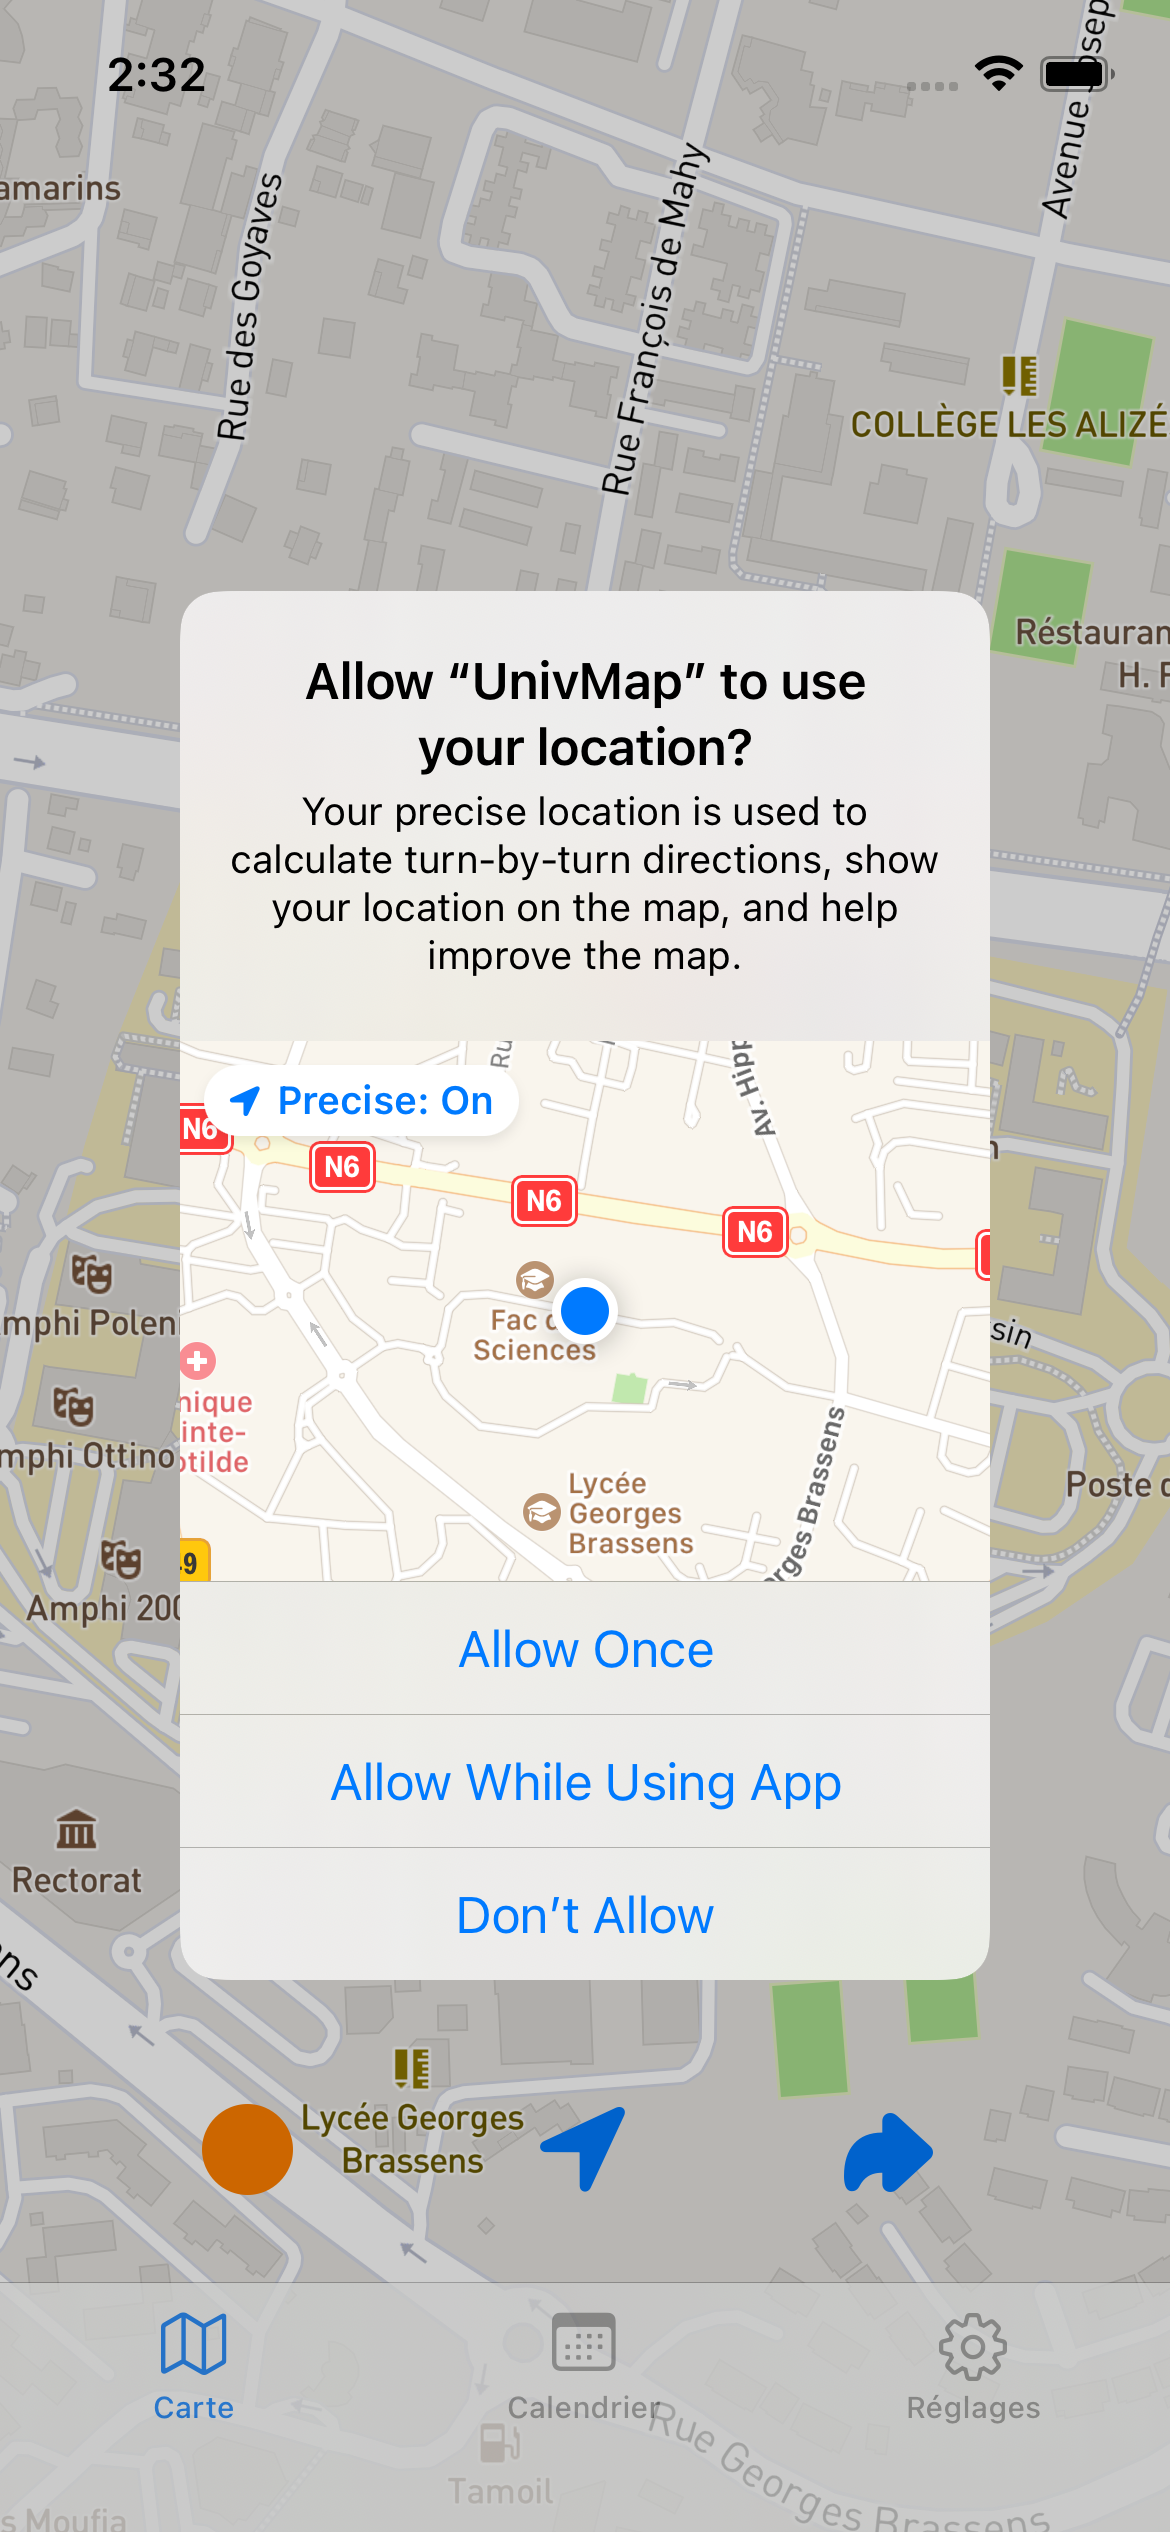
\includegraphics[width=30mm, scale=0.5]{allowUserLocation.png}
      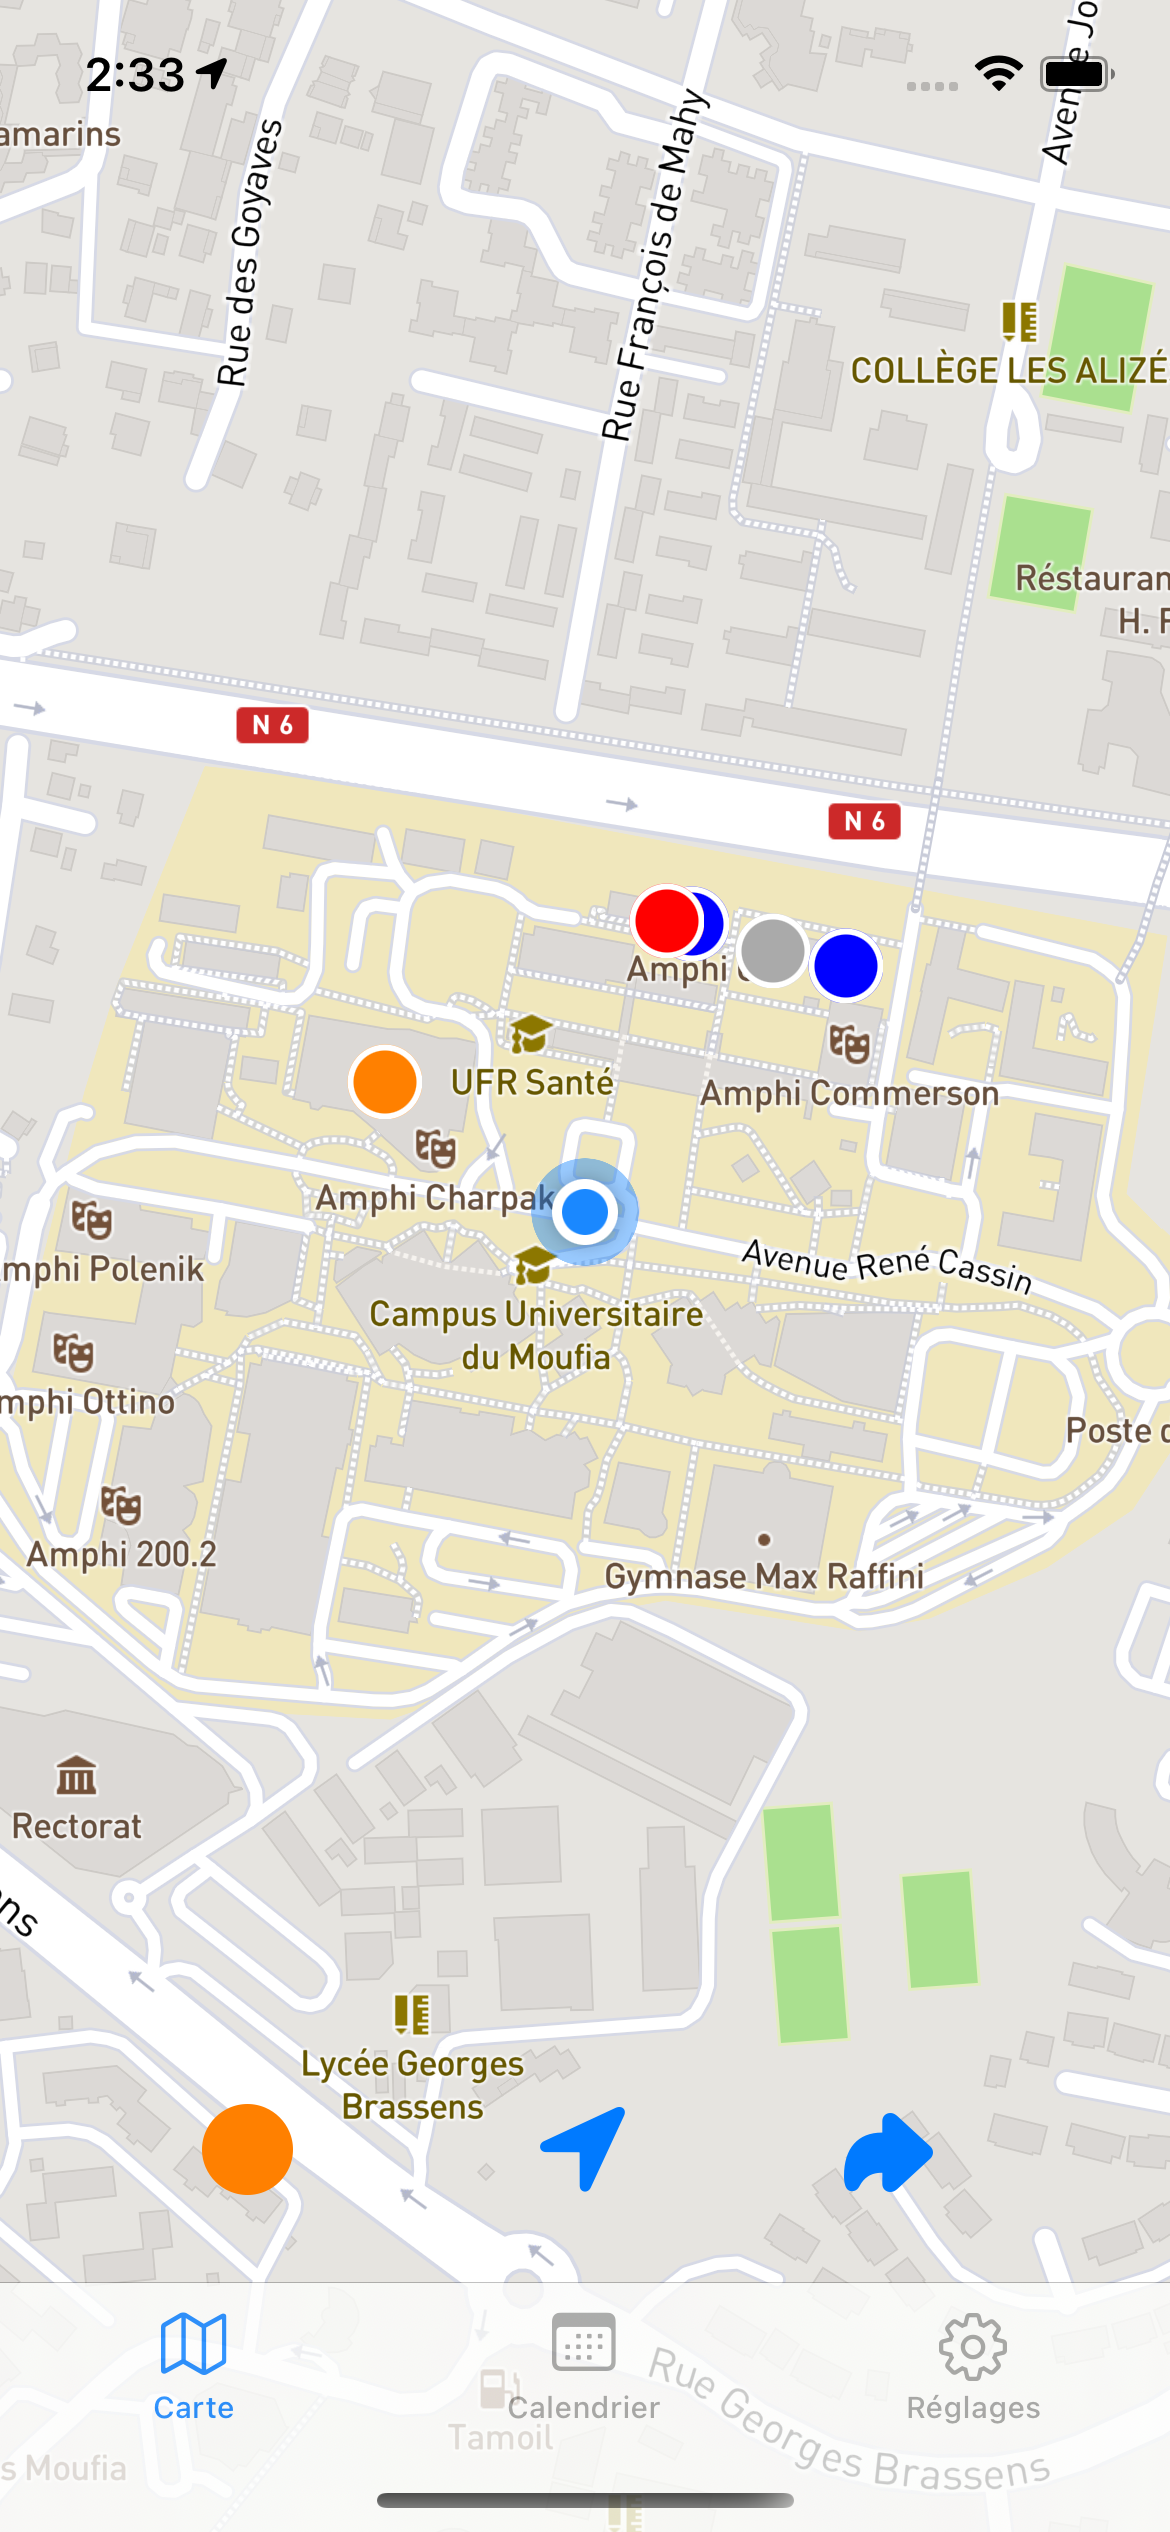
\includegraphics[width=30mm, scale=0.5]{map.png}
      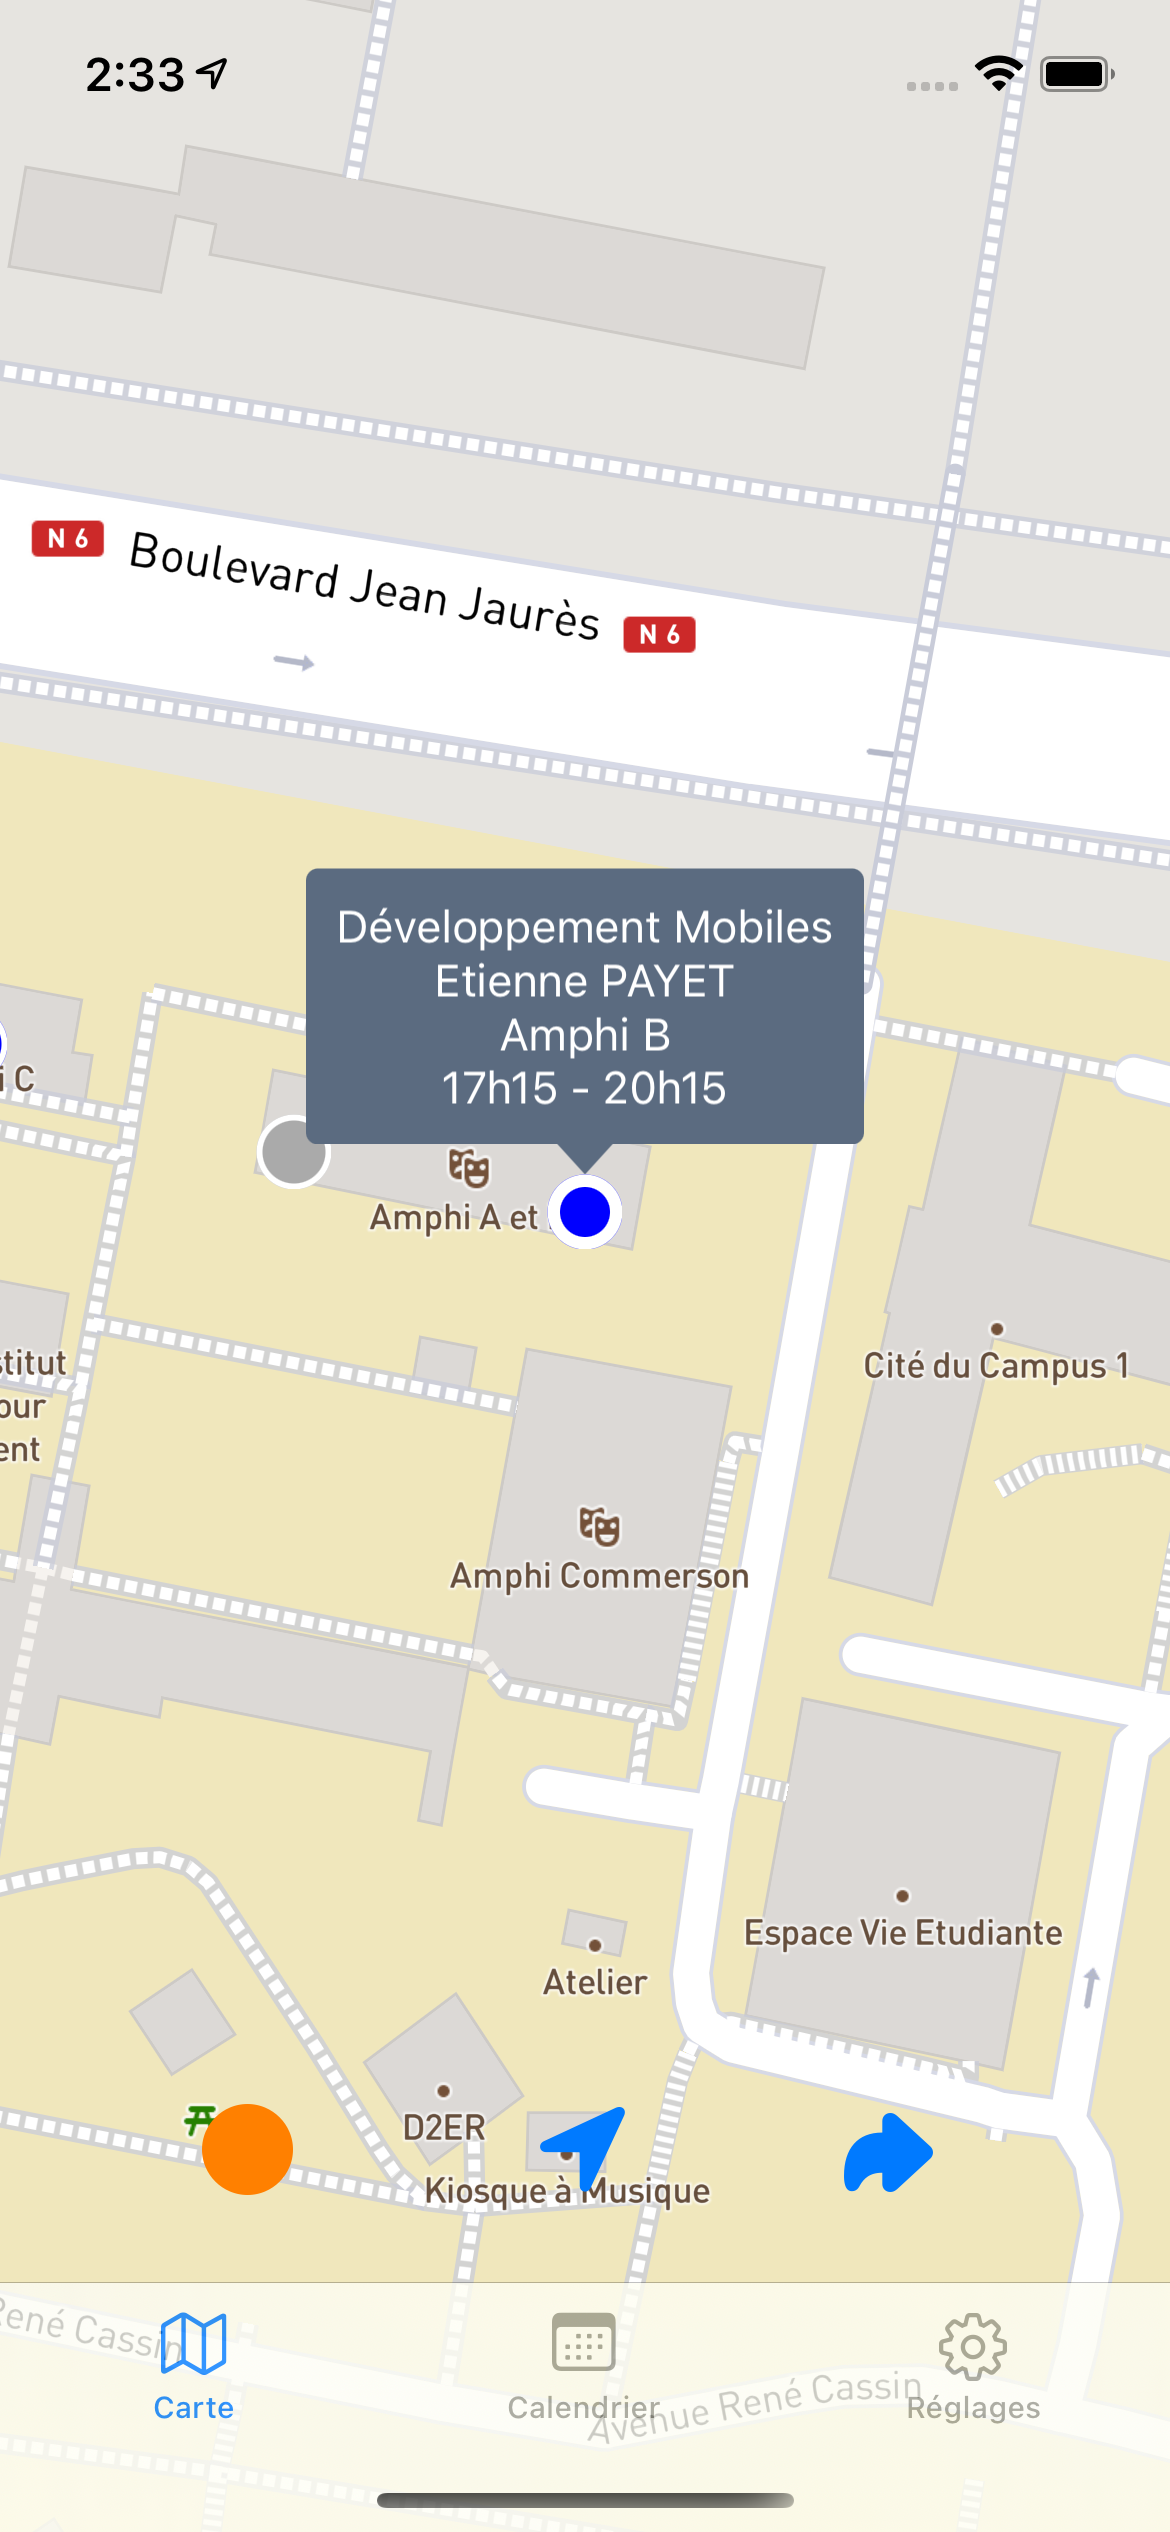
\includegraphics[width=30mm, scale=0.5]{point_bleu.png}
    \end{center}
  \end{frame}


  \begin{frame}
    \frametitle{Comment fontionne : le calendrier}
    \begin{center}
      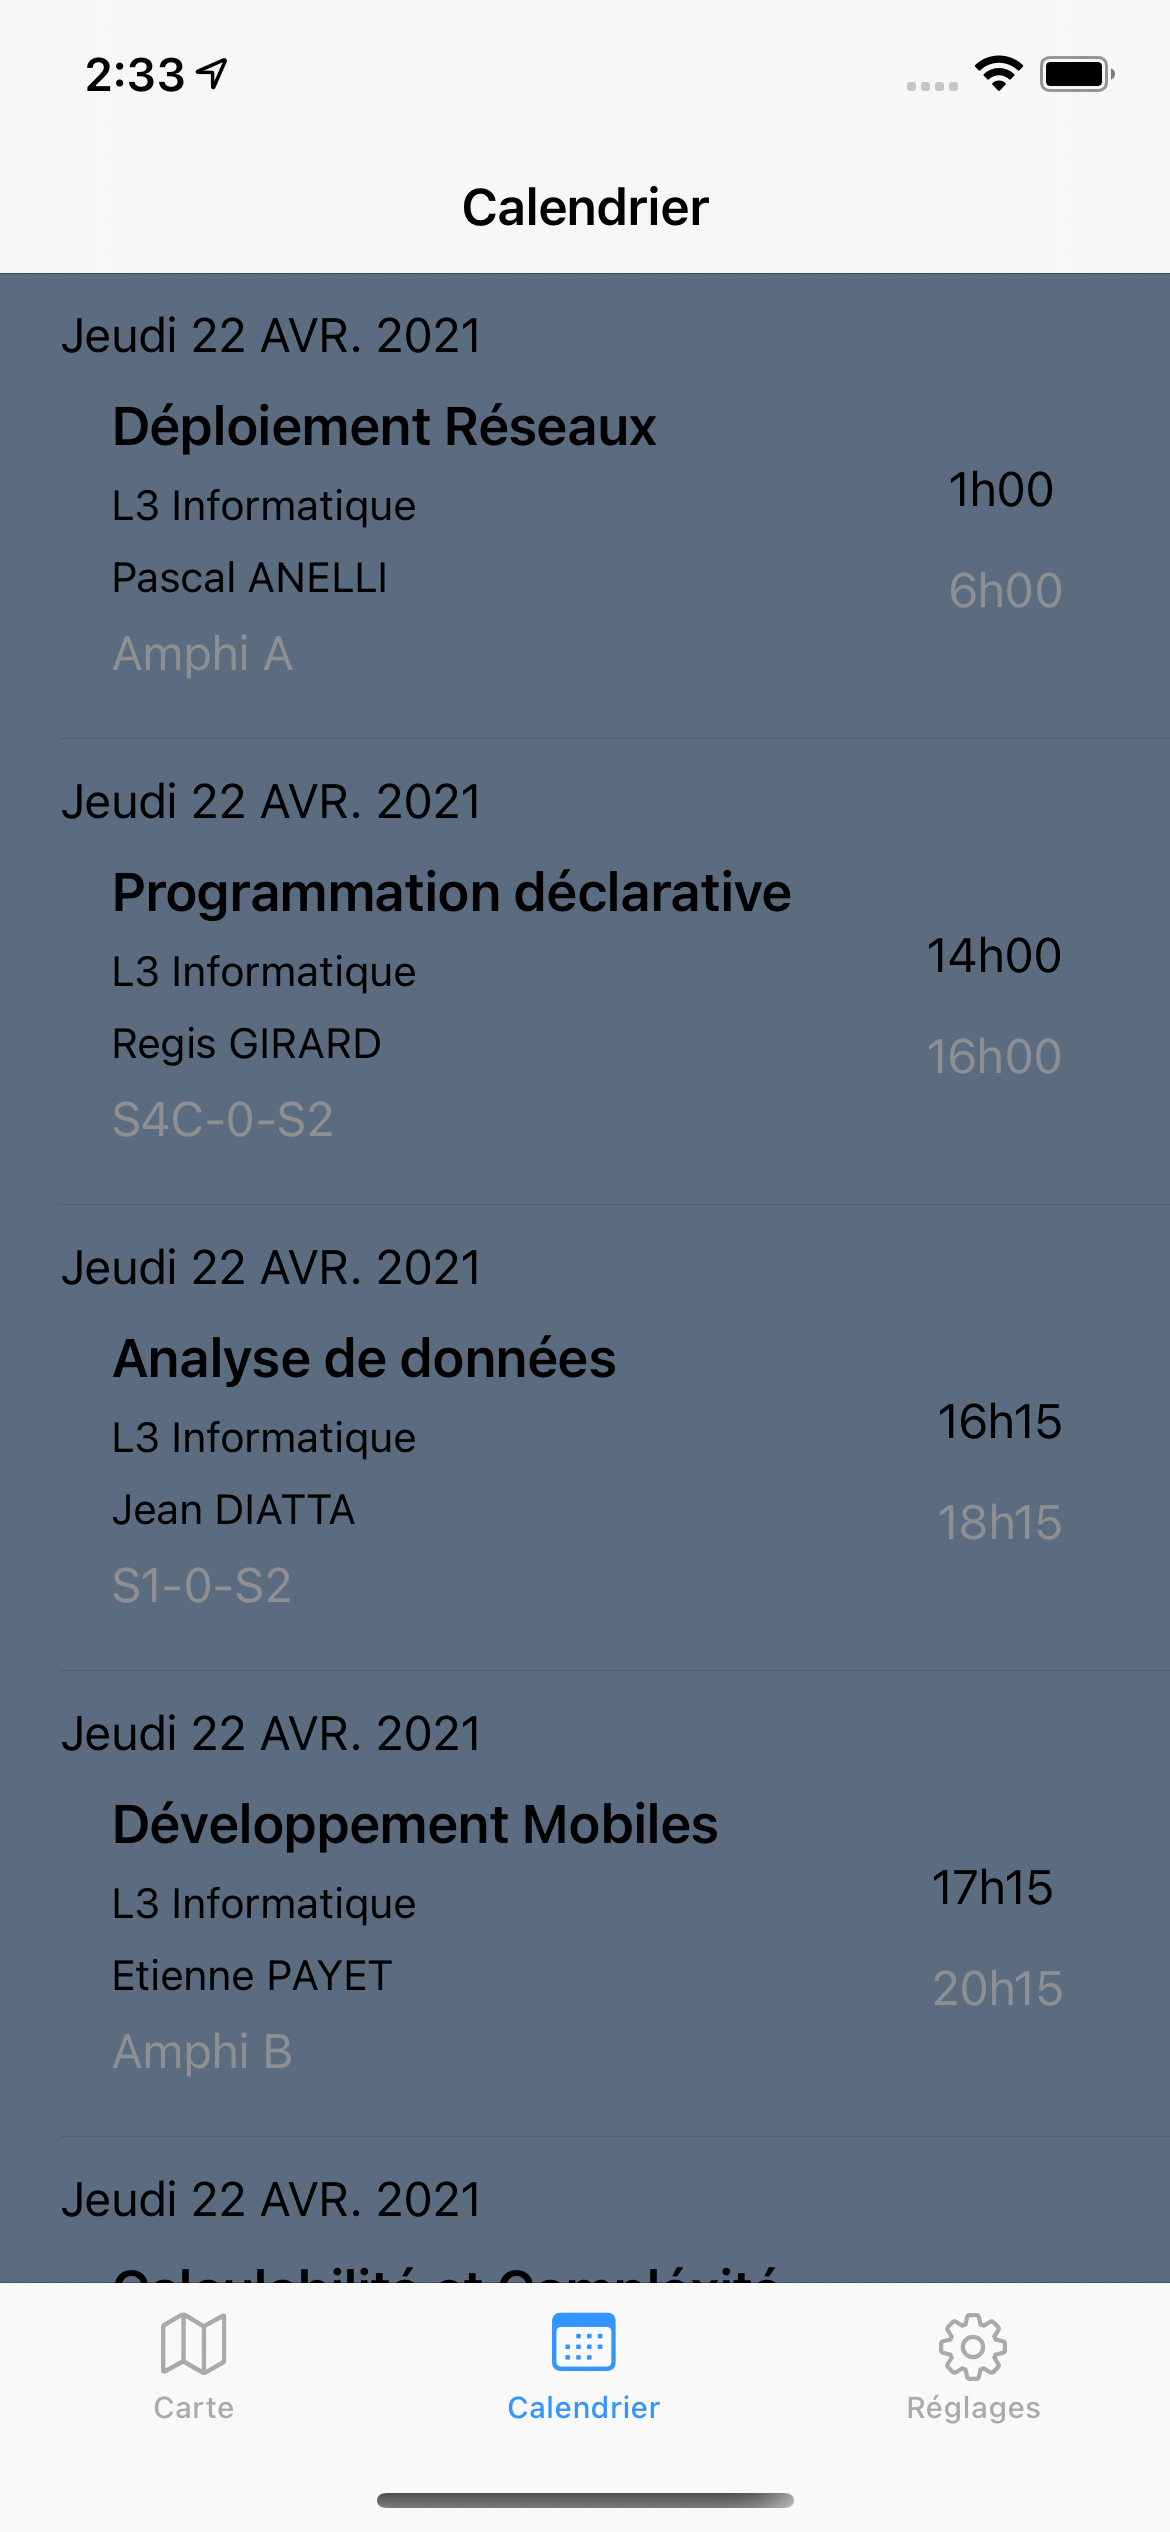
\includegraphics[width=30mm, scale=0.5]{calendar.png}
      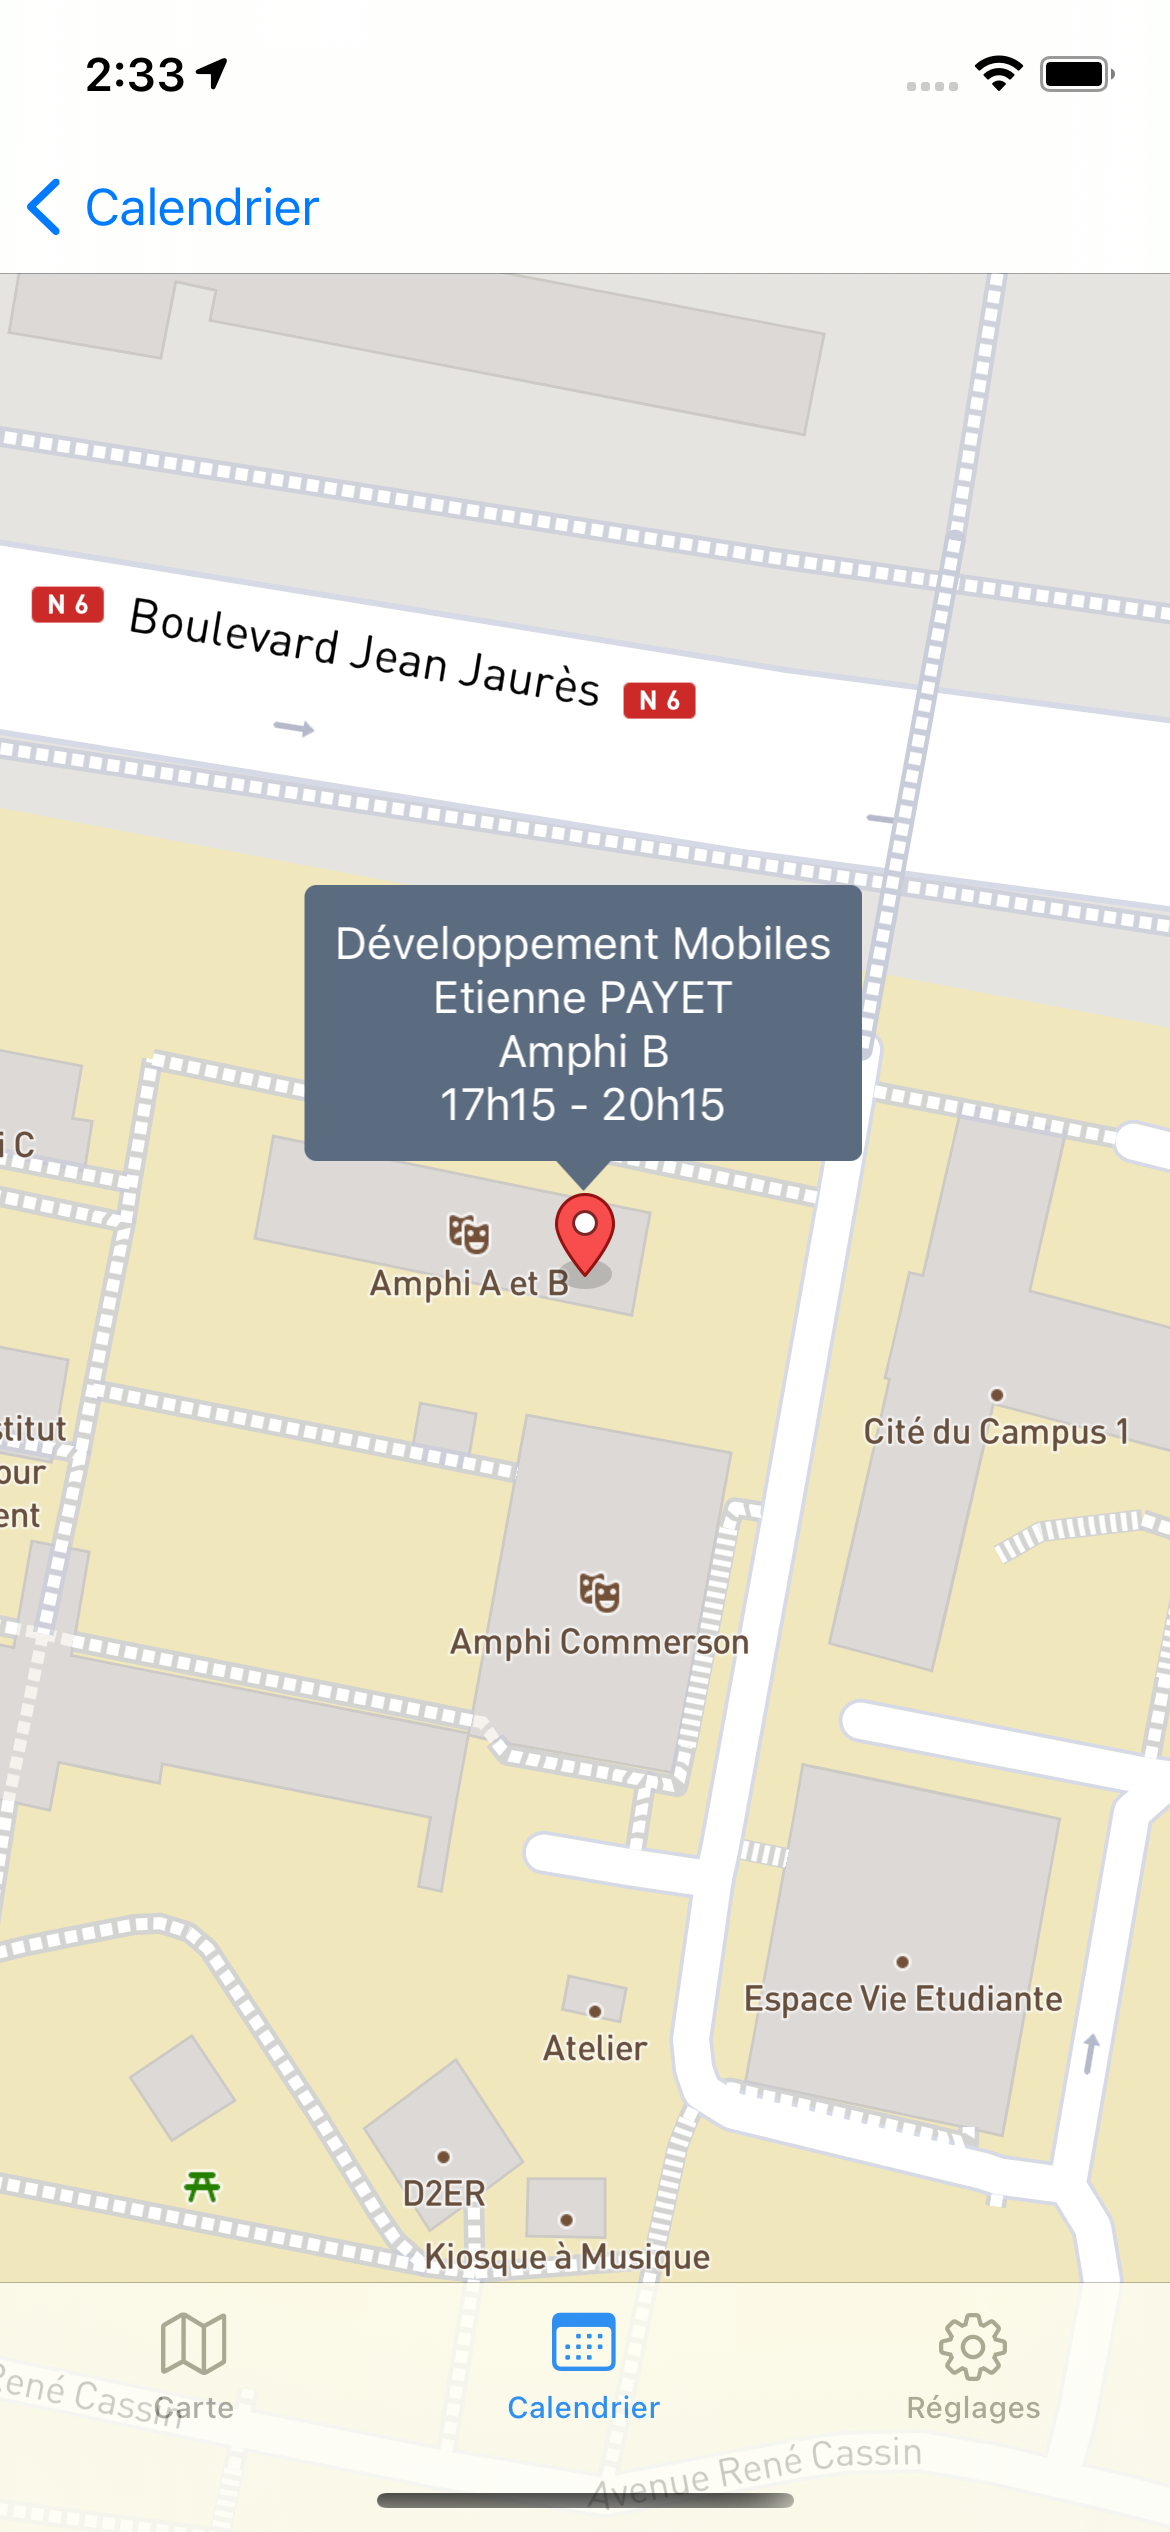
\includegraphics[width=30mm, scale=0.5]{calendar_position.png}
    \end{center}
  \end{frame}


  \begin{frame}
    \frametitle{Comment fontionne : les paramètres}
    \begin{center}
      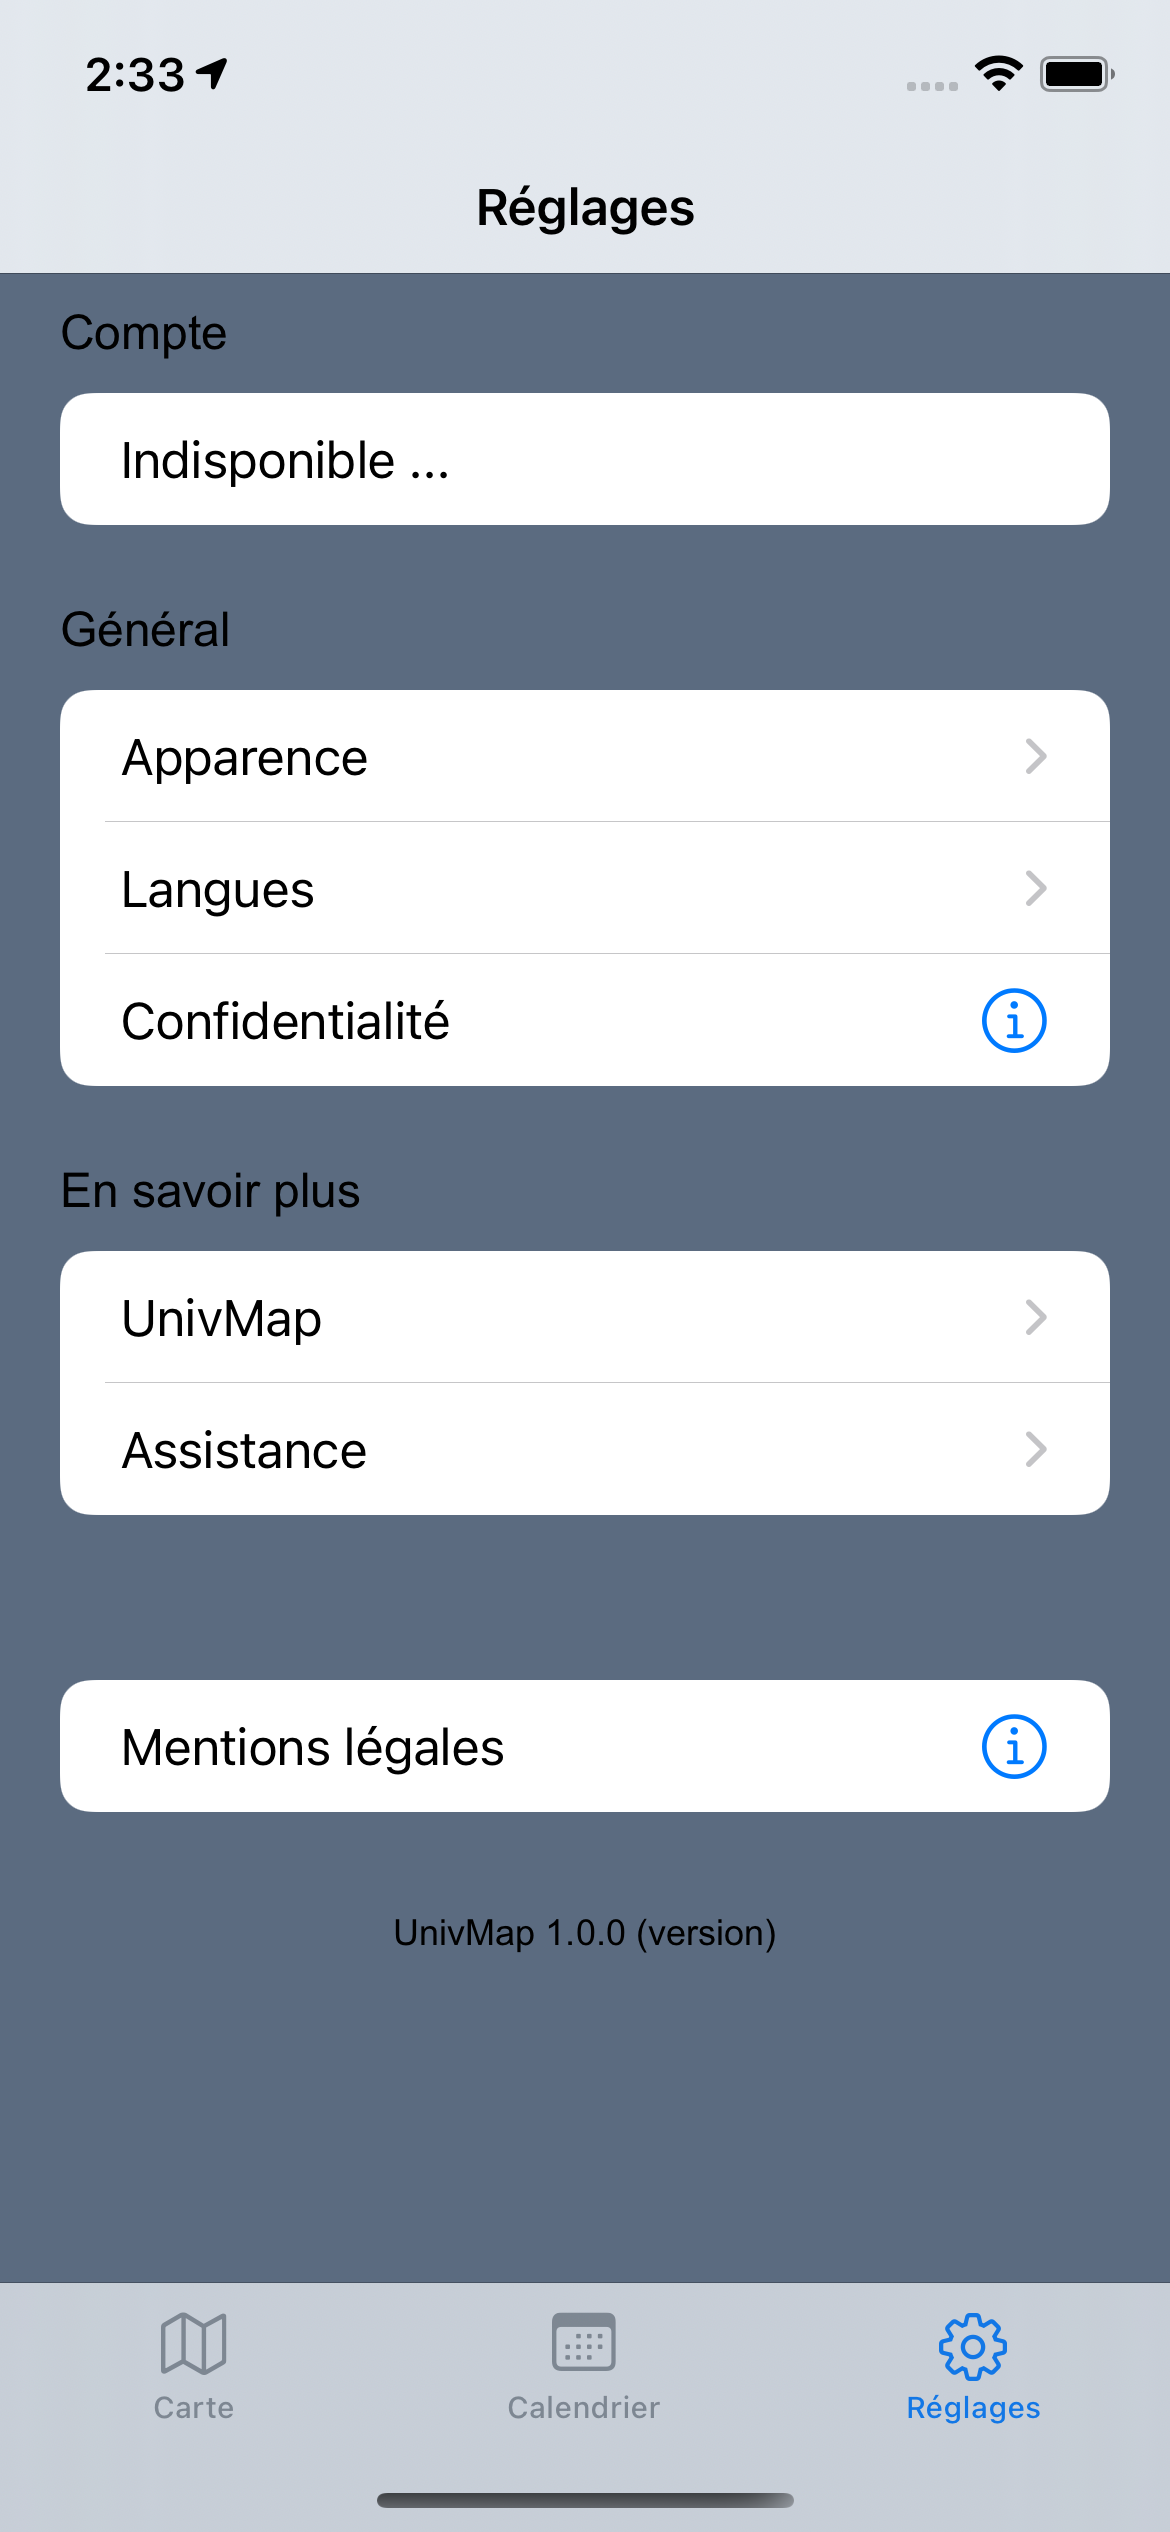
\includegraphics[width=30mm, scale=0.5]{setting.png}
      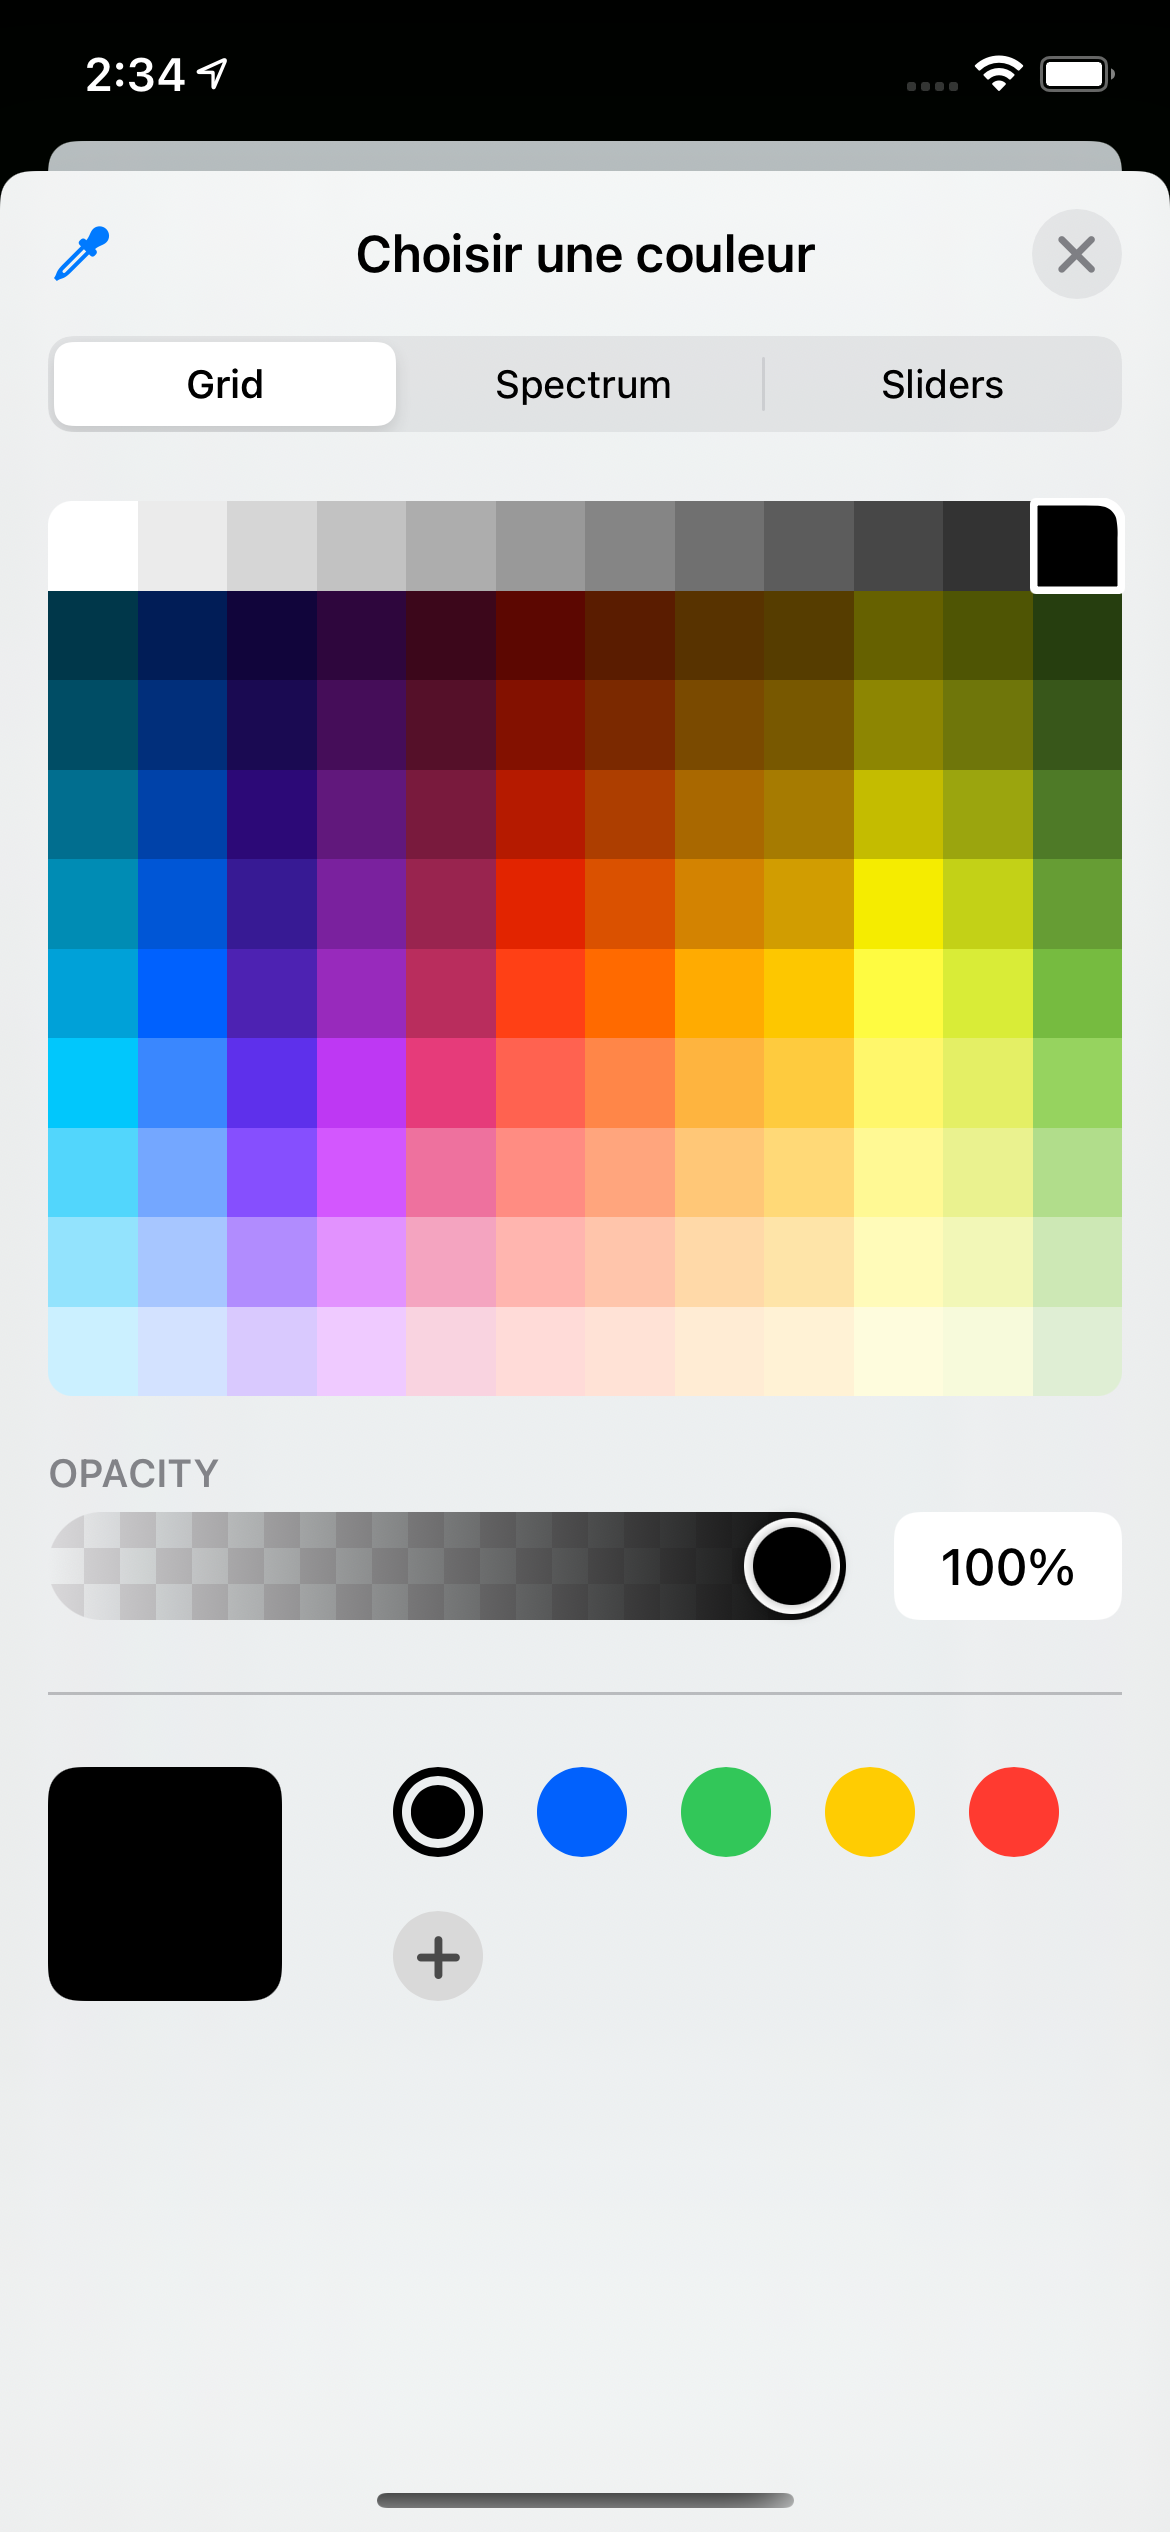
\includegraphics[width=30mm, scale=0.5]{setting_appearance.png}
      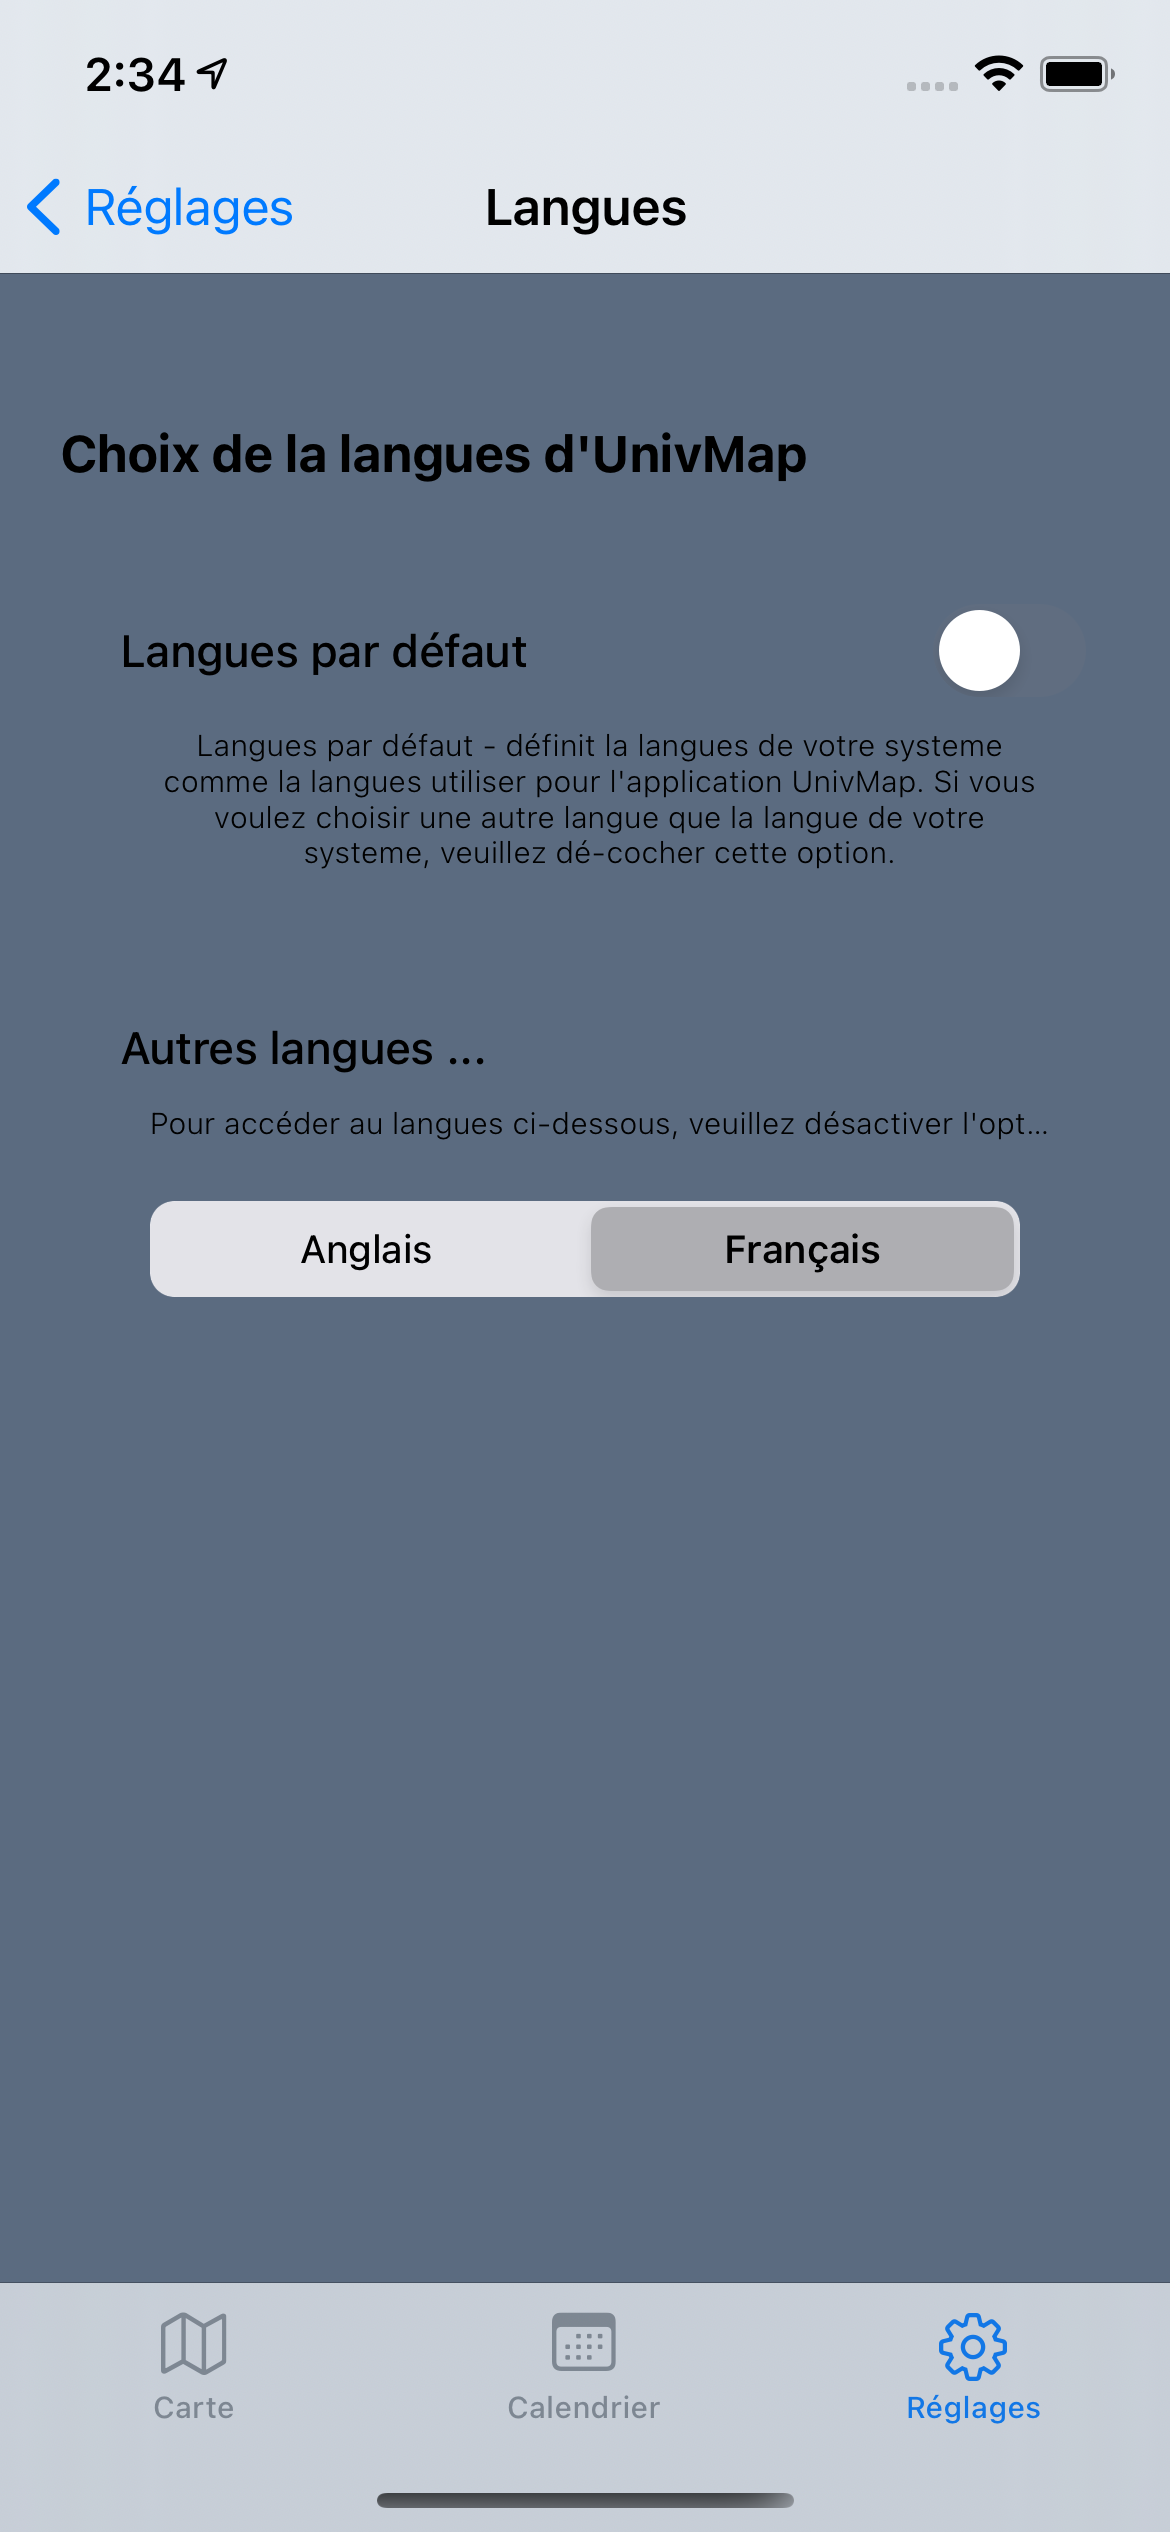
\includegraphics[width=30mm, scale=0.5]{setting_languageOff.png}
    \end{center}
  \end{frame}
%
%
%%%%%%%%%%%%%%%%%%%%%%%%%%%%%%%%%%%%%%%%%%%%%%%%%%%%%%%%%%%%%%%%%%%%%%%%%%%%%
\section{Composantes utilisés}
%%%%%%%%%%%%%%%%%%%%%%%%%%%%%%%%%%%%%%%%%%%%%%%%%%%%%%%%%%%%%%%%%%%%%%%%%%%%%
%
%
\subsection{Mapbox}
  \begin{frame}
    \frametitle{Mapbox : c'est quoi ?}

    \begin{itemize}
      \item Entreprise américaine spécialisée dans la cartographie en ligne
      \item Mapbox reposent principalement sur le logiciel libre et sur les données d'OpenStreetMap
      \item Fournis ses services notamment à :
      \begin{itemize}
        \item Pinterest
        \item Le Monde
        \item Snapchat
        \item ...
      \end{itemize}
    \end{itemize}

  \end{frame}

    

\subsection{Firebase}
  \begin{frame}
    \frametitle{Firebase : c'est quoi ?}

    \begin{itemize}
      \item Services d'hébergement pour tout type d'application
      \item Racheté par Google en 2014
      \item Firebase : NoSQL
      \item Utilisé par plus de 110 000 développeurs :
      \begin{itemize}
        \item Shazam (iOS et Android)
        \item Le Figaro (iOS et Android)
        \item ...
      \end{itemize}
    \end{itemize}

  \end{frame}

  \begin{frame}
    \frametitle{Firebase : c'est quoi ?}

    \begin{center}
      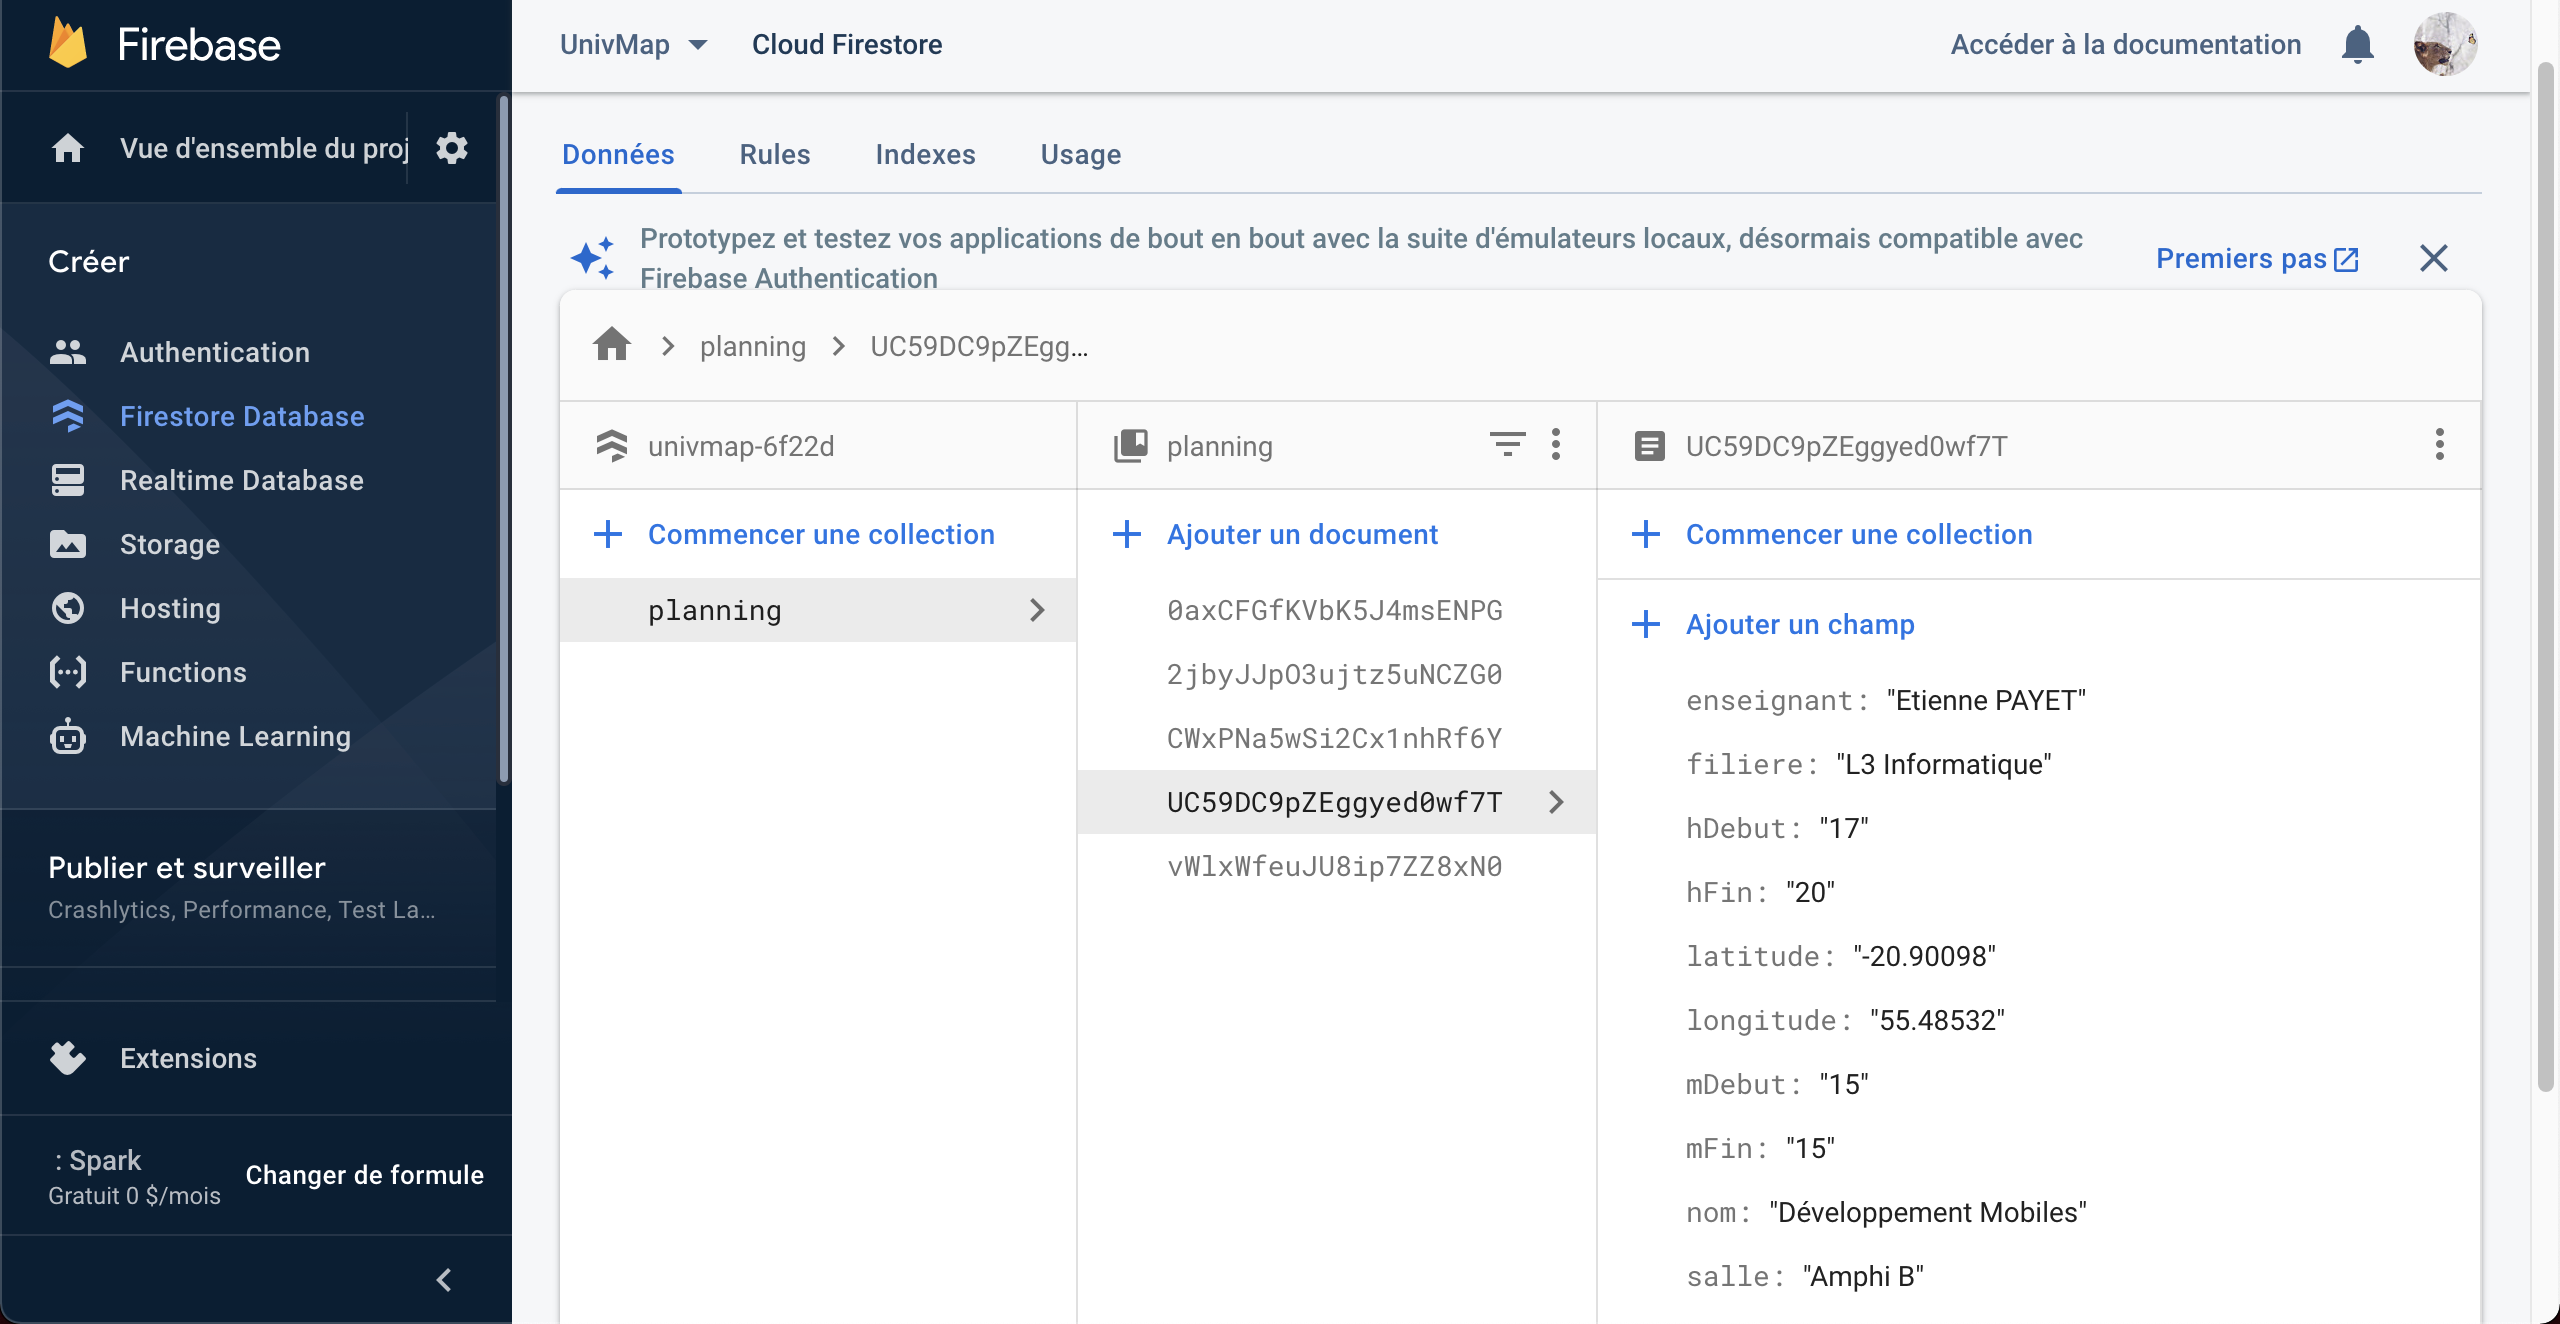
\includegraphics[width=120mm, scale=0.5]{firebase.png}
    \end{center}

  \end{frame}


%
%
%%%%%%%%%%%%%%%%%%%%%%%%%%%%%%%%%%%%%%%%%%%%%%%%%%%%%%%%%%%%%%%%%%%%%%%%%%%%%
\section{Quelques difficultés}
%%%%%%%%%%%%%%%%%%%%%%%%%%%%%%%%%%%%%%%%%%%%%%%%%%%%%%%%%%%%%%%%%%%%%%%%%%%%%
%
%
\begin{frame}
  \frametitle{Quelques difficultés}
  \begin{itemize}
    \item Apprendre l'utilisation des API
    \item Comprendre les documentations
    \item Prise en main de Git
    \item Changement de langues sur iOS
  \end{itemize}
\end{frame}
%
%
%%%%%%%%%%%%%%%%%%%%%%%%%%%%%%%%%%%%%%%%%%%%%%%%%%%%%%%%%%%%%%%%%%%%%%%%%%%%%
\section{UnivMap 2.0 : À Suivre}
%%%%%%%%%%%%%%%%%%%%%%%%%%%%%%%%%%%%%%%%%%%%%%%%%%%%%%%%%%%%%%%%%%%%%%%%%%%%%
%
%
\begin{frame}
  \frametitle{UnivMap 2.0 : À Suivre}

  \begin{itemize}
    \item Choix du planning selon une filière
    \item Notification losque l'emploi du temps est modifié
    \item Un onglet accueil afin d'être redirigé vers d'autres plateformes de l'Université
    \item Ajout de filtre pour la carte pour n'afficher que le contenu voulu
    \item Un système permettant de rechercher des salles
  \end{itemize}


\end{frame}
%
%
%%%%%%%%%%%%%%%%%%%%%%%%%%%%%%%%%%%%%%%%%%%%%%%%%%%%%%%%%%%%%%%%%%%%%%%%%%%%%
\section{Conclusion}
%%%%%%%%%%%%%%%%%%%%%%%%%%%%%%%%%%%%%%%%%%%%%%%%%%%%%%%%%%%%%%%%%%%%%%%%%%%%%
%
%
\begin{frame}
  \frametitle{Conclusion}

  \begin{center}
    
\includegraphics[width=35mm, scale=0.5]{UnivMap-logo500x500.png}
  \end{center}

  \begin{itemize}
    \item Appréhension sur l'idée de l'application
    \item Travail de groupe : communication, entraide étaient très important
    \item L'ambition et la persévérance d'atteindre cette objectif
  \end{itemize}
\end{frame}
%
%
\end{document}
